\documentclass[12pt]{article}

\usepackage[margin=1in]{geometry}
\usepackage{amsmath,amssymb,amsthm}
\usepackage{enumitem}
\usepackage{booktabs}
\usepackage{tabularx}
\usepackage{hyperref}
\usepackage{graphicx}
\usepackage{tikz}
\usetikzlibrary{decorations.pathreplacing,positioning}

\newtheorem{theorem}{Theorem}
\newtheorem{proposition}{Proposition}

\title{A Two-Pole Construction of Second-Order Linear ODEs\\
with Degree-2 Liouvillian Solutions}
\author{
  Brodie Foxworth\thanks{Independent researcher; \href{https://pottersquill.com}{Potter's Quill Publishing}} \quad
  Mark F. Kruelle\thanks{Yale Alumni; \href{https://pottersquill.com}{Potter's Quill Publishing}} \quad
  Kevin D. Potter\thanks{Saint Leo Alumni; \href{https://pottersquill.com}{Potter's Quill Publishing}}
}
\date{}

\begin{document}
\maketitle

\begin{abstract}
We present a systematic construction of a family of second-order linear ODEs of the form
\[
  y'' + r(z)\,y = 0
\]
whose solutions are Liouvillian and arise from a logarithmic derivative
$s(z) \in \mathbb{C}(z,\sqrt{R})$ of algebraic degree exactly~2 over $\mathbb{C}(z)$.
The construction places two poles at $z=0$ and $z=1$ with equal residues $\tfrac{1}{4}$,
yielding the potential $r(z) = \frac{3}{16\,{z^2}(z-1)^2}$ and solutions expressible
in terms of radicals and inverse hyperbolic functions. We verify the Riccati equation
by direct computation, prove that the logarithmic derivative has algebraic degree~2
via its minimal polynomial, and establish linear independence of the two fundamental
solutions via their nonconstant ratio and constant Wronskian. A generalization to
$n$ poles is outlined. We have not found this two-pole construction in the standard
references consulted.
\end{abstract}

\section{Introduction}

The Kovacic algorithm~\cite{kovacic} provides a systematic method for determining whether a
second-order linear ODE of the form
\begin{equation}
  y'' + r(z)\,y = 0
  \label{eq:ode}
\end{equation}
has Liouvillian solutions, i.e., solutions expressible in terms of exponentials, logarithms,
and algebraic functions. The algorithm operates by examining the poles of the coefficient
function $r(z)$ and classifying the local behavior at each singular point into one of four
cases, each of which constrains the possible algebraic degree of the logarithmic derivative
of a solution.

A Liouvillian solution of \eqref{eq:ode} can be written as $y_1 = \exp\!\bigl(\int s(z)\,dz\bigr)$,
where $s(z) \in \mathbb{C}(z,\sqrt{R})$ satisfies the Riccati equation
\begin{equation}
  s' + s^2 + r(z) = 0.
  \label{eq:riccati}
\end{equation}
The algebraic degree of $s(z)$ over $\mathbb{C}(z)$ determines the complexity of the solution.
Kovacic's algorithm searches for $s(z)$ of degree 1, 2, 4, or 8 over $\mathbb{C}(z)$.
In this paper, we focus on degree-2 solutions, where $s(z) \in \mathbb{C}(z,\sqrt{R})$
for some square-free $R \in \mathbb{C}(z)$ with $\sqrt{R} \notin \mathbb{C}(z)$.

We present a construction that starts from the desired algebraic structure---a quadratic
extension $\mathbb{C}(z,\sqrt{R})/\mathbb{C}(z)$---and derives the ODE coefficient $r(z)$
from the Riccati equation. This is the reverse of the usual approach, which starts from
$r(z)$ and attempts to find $s(z)$. Our construction naturally produces ODEs with two poles,
in contrast to many of the single-pole or single-point examples we encountered in the
references consulted within Kovacic's framework.

\section{The Two-Pole Ansatz}

We seek a logarithmic derivative of the form
\begin{equation}
  s(z) = A(z) + B(z)\,\sqrt{R(z)}, \quad A,B,R \in \mathbb{C}(z),\; \sqrt{R}\notin\mathbb{C}(z),
  \label{eq:sdef}
\end{equation}
where $A, B, R \in \mathbb{C}(z)$ and $\sqrt{R} \notin \mathbb{C}(z)$. The function $s(z)$
lies in the quadratic extension $\mathbb{C}(z,\sqrt{R})$ of $\mathbb{C}(z)$. The Riccati
equation $s' + s^2 + r(z) = 0$ implies
\[
  r(z) = -(s' + s^2).
\]

We place two poles at $z=0$ and $z=1$ with equal residues $\tfrac{1}{4}$. This gives:
\begin{align}
  A(z) &= \frac{2z-1}{4\,z(z-1)} = \frac{1}{4z} + \frac{1}{4(z-1)}, \label{eq:Adef} \\
  R(z) &= \frac{1}{z(z-1)}, \label{eq:Rdef} \\
  B &= c = \tfrac{1}{2}. \label{eq:Bval}
\end{align}
The choice $B = c = \tfrac{1}{2}$ (constant) is the simplest case of the general framework
where $B = c \cdot f(z)$ for some $f(z) \in \mathbb{C}(z)$. Note that $B$ is a free
parameter: the irrational cancellation condition $\frac{R'}{2} + 2AR = 0$ is independent
of $B$. For $f(z) = 1$ (constant), this cancellation is an algebraic identity (verified
by logarithmic differentiation of $R = \prod(z-z_i)^{-n_i}$), but for general $f(z)$,
additional constraints are needed to ensure $r(z) \in \mathbb{C}(z)$; this case is left
for future work. Note that while the cancellation condition is independent of $B$, the resulting
potential $r(z)$ depends on $B^2$. The choice $B = \tfrac{1}{2}$ gives the simple potential used in the two-pole
example above. For the simplest subfamily
$f(z)=1$, the constraint gives $B = c$, a constant. This yields the two branches:
\begin{equation}
  s_{\pm}(z) = \frac{2z-1}{4\,z(z-1)} \pm \frac{1}{2\sqrt{z(z-1)}}.
  \label{eq:spm}
\end{equation}

The two poles of $A$ are located at $z=0$ and $z=1$, each with residue $\tfrac{1}{4}$;
the branch cut for $\sqrt{z(z-1)}$ is taken along $[0,1]$.

\subsection{Field-Extension Tower}

\begin{center}
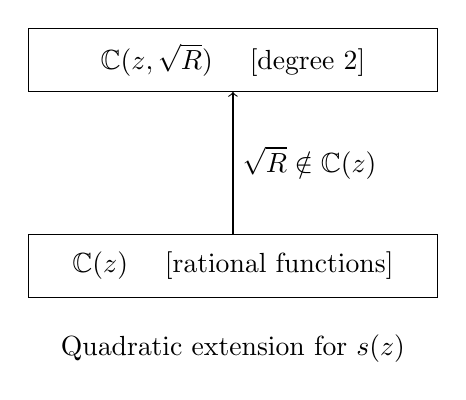
\begin{tikzpicture}[node distance=1.8cm]
\node[draw, minimum width=5.2cm, minimum height=0.8cm, align=center] (top)
  {$\mathbb{C}(z,\sqrt{R})$ \quad [degree 2]};
\node[draw, below=of top, minimum width=5.2cm, minimum height=0.8cm, align=center] (bottom)
  {$\mathbb{C}(z)$ \quad [rational functions]};
\draw[->] (bottom) -- (top)
  node[midway, right] {$\sqrt{R} \notin \mathbb{C}(z)$};
\node[below=0.35cm of bottom] {Quadratic extension for $s(z)$};
\end{tikzpicture}
\end{center}

\section{The Construction}

\subsection{Choosing the Poles and Computing $A$, $B$, $R$, $s$}

We choose poles at $z_1=0$ and $z_2=1$ with residues $a_1=a_2=\tfrac{1}{4}$
(corresponding to $n_1=n_2=1$, both odd). The partial-fraction decomposition of $A$ is:
\[
  A(z) = \frac{2z-1}{4\,z(z-1)} = \frac{1}{4z} + \frac{1}{4(z-1)}.
\]
The radicand $R$ encodes the irrational part of the logarithmic derivative:
\[
  R(z) = \frac{1}{z(z-1)}.
\]
With $B = c = \tfrac{1}{2}$ (the simplest subfamily, $f(z)=1$), the two branches of the
logarithmic derivative are:
\[
  s_{\pm}(z) = \frac{2z-1}{4\,z(z-1)} \pm \frac{1}{2\sqrt{z(z-1)}}.
\]

\section{The ODE and Its Solutions}

\subsection{The Potential $r(z)$}

From the Riccati equation, $r(z) = -(s' + s^2)$. We first compute the rational part
$A' + A^2 + B^2 R$. The irrational part is shown below to vanish for this choice of $A$
and $R$:
\begin{align}
  A' &= -\frac{1}{4z^2} - \frac{1}{4(z-1)^2}, \label{eq:Ap} \\
  A^2 &= \frac{1}{16z^2} + \frac{1}{8\,z(z-1)} + \frac{1}{16(z-1)^2}, \label{eq:Asq} \\
  B^2 R &= \frac{1}{4\,z(z-1)}. \label{eq:B2R}
\end{align}
Summing these three contributions:
\begin{equation}
  A' + A^2 + B^2 R = -\frac{3}{16z^2} - \frac{3}{16(z-1)^2} + \frac{3}{8\,z(z-1)}
  = -\frac{3}{16\,z^2(z-1)^2}.
  \label{eq:sumABR}
\end{equation}
Therefore:
\begin{equation}
  r(z) = -(A' + A^2 + B^2 R) = \frac{3}{16\,z^2(z-1)^2}.
  \label{eq:rresult}
\end{equation}
The irrational parts cancel because $\frac{R'}{2} + 2AR = 0$ for our specific $A$ and $R$
(verified explicitly in Theorem~\ref{thm:riccati}), so both branches yield the same
$r(z) \in \mathbb{C}(z)$. This is a necessary condition for the construction to produce a
rational ODE coefficient.

\subsection{Integrating $s$ to Obtain $y_1$}

The first solution is $y_1 = \exp\!\bigl(\int s_+\,dz\bigr)$. We split the integral:
\begin{equation}
  \int s_+\,dz = \int \frac{2z-1}{4\,z(z-1)}\,dz + \int \frac{1}{2\sqrt{z(z-1)}}\,dz.
  \label{eq:int1}
\end{equation}
The first integral is elementary:
\begin{equation}
  = \tfrac{1}{4}\ln\!\bigl(z(z-1)\bigr) + \tfrac{1}{2}\,\operatorname{arcosh}(2z-1).
  \label{eq:int2}
\end{equation}
Using $\operatorname{arcosh}(2z-1) = \ln\!\bigl(2z-1 + 2\sqrt{z(z-1)}\bigr)$
(valid as a complex identity, with branch cut $[0,1]$ corresponding to the
branch cut of $\sqrt{z(z-1)}$), we obtain:
\begin{equation}
  = \tfrac{1}{4}\ln\!\bigl(z(z-1)\bigr) + \tfrac{1}{2}\ln\!\bigl(2z-1 + 2\sqrt{z(z-1)}\bigr).
  \label{eq:int3}
\end{equation}
Exponentiating:
\begin{equation}
  y_1 = \bigl[z(z-1)\bigr]^{1/4}\,\bigl[2z-1 + 2\sqrt{z(z-1)}\bigr]^{1/2}.
  \label{eq:y1}
\end{equation}

\subsection{The Second Solution $y_2$ from the Conjugate}

The second solution $y_2$ arises from the conjugate logarithmic derivative
\begin{equation}
  s_2 = A - B\sqrt{R},
  \label{eq:s2def}
\end{equation}
obtained by applying the nontrivial automorphism of the quadratic extension
$\mathbb{C}(z,\sqrt{R})/\mathbb{C}(z)$, which sends $\sqrt{R} \mapsto -\sqrt{R}$.
This yields:
\begin{equation}
  y_2 = \bigl[z(z-1)\bigr]^{1/4}\,\bigl[2z-1 - 2\sqrt{z(z-1)}\bigr]^{1/2}.
  \label{eq:y2}
\end{equation}
The automorphism preserves the Riccati equation (since $r(z) \in \mathbb{C}(z)$ is fixed),
so $s_2$ is also a root, and $y_2 = \exp\!\bigl(\int s_2\,dz\bigr)$ is also a solution.

\section{Proofs}

\begin{theorem}[Riccati Verification]
\label{thm:riccati}
Let $A(z) = \frac{2z-1}{4\,z(z-1)}$, $B = \frac{1}{2}$, $R(z) = \frac{1}{z(z-1)}$, and
$s_{\pm} = A \pm B\sqrt{R}$. Define $r(z) = -(A' + A^2 + B^2 R)$. Then
$r(z) = \frac{3}{16\,z^2(z-1)^2}$, and both $s_+$, $s_-$ satisfy the Riccati equation
$s' + s^2 + r(z) = 0$.
\end{theorem}

\begin{proof}
We compute each term separately.

\textbf{Derivative of $A$:} Since $A = \frac{1}{4z} + \frac{1}{4(z-1)}$, we have
\[
  A' = -\frac{1}{4z^2} - \frac{1}{4(z-1)^2}.
\]

\textbf{Square of $A$:}
\[
  A^2 = \frac{1}{16z^2} + \frac{1}{8\,z(z-1)} + \frac{1}{16(z-1)^2}.
\]

\textbf{$B^2 R$:} With $B = \tfrac{1}{2}$ and $R = \frac{1}{z(z-1)}$:
\[
  B^2 R = \frac{1}{4\,z(z-1)}.
\]

\textbf{Sum:}
\[
  A' + A^2 + B^2 R = -\frac{3}{16\,z^2(z-1)^2}.
\]
Therefore:
\[
  r(z) = -(A' + A^2 + B^2 R) = \frac{3}{16\,z^2(z-1)^2}.
\]

To verify that $s_+$ satisfies the Riccati equation, note that $s_+ = A + B\sqrt{R}$, so
\[
  s_+' + s_+^2 = (A' + A^2 + B^2 R) + \left(\frac{B\,R'}{2\sqrt{R}} + 2AB\sqrt{R}\right).
\]
The irrational part is $\frac{B}{\sqrt{R}}\left(\frac{R'}{2} + 2AR\right)$.
For our specific $A$ and $R$:
\[
  \frac{R'}{2} + 2AR = \frac{-(2z-1)}{2\,z^2(z-1)^2} + \frac{2(2z-1)}{4\,z(z-1)} \cdot \frac{1}{z(z-1)}
  = \frac{-(2z-1)}{2\,z^2(z-1)^2} + \frac{(2z-1)}{2\,z^2(z-1)^2} = 0.
\]
Thus the irrational part vanishes, and $s' + s^2 = A' + A^2 + B^2 R = -r(z)$.
The case $s_- = A - B\sqrt{R}$ is identical with $B$ replaced by $-B$; since the
irrational term is proportional to $B$ and equals zero, both branches satisfy the
Riccati equation.
\end{proof}

\begin{theorem}[Algebraic Degree~2]
\label{thm:degree2}
The logarithmic derivative $s = A + B\sqrt{R}$ has algebraic degree exactly~2 over
$\mathbb{C}(z)$, i.e., $s \notin \mathbb{C}(z)$ and $s$ satisfies a degree-2 minimal
polynomial over $\mathbb{C}(z)$.
\end{theorem}

\begin{proof}
Since $s = A + B\sqrt{R}$ with $B \neq 0$ and $\sqrt{R} \notin \mathbb{C}(z)$, we have
$s \notin \mathbb{C}(z)$. The minimal polynomial of $s$ over $\mathbb{C}(z)$ is obtained
by eliminating $\sqrt{R}$ from $s = A + B\sqrt{R}$:
\[
  (s - A)^2 = B^2 R, \quad\text{i.e.,}\quad s^2 - 2As + (A^2 - B^2 R) = 0.
\]
Substituting $A = \frac{2z-1}{4\,z(z-1)}$, $B = \tfrac{1}{2}$, $R = \frac{1}{z(z-1)}$:
\[
  s^2 - \frac{2z-1}{2\,z(z-1)}\,s + \frac{1}{16\,z^2(z-1)^2} = 0.
\]
Here $R = \frac{1}{z(z-1)}$ is not a square in $\mathbb{C}(z)$, since it has
simple poles at $z=0$ and $z=1$ (a square in $\mathbb{C}(z)$ can only have even-order
poles). Since $\sqrt{R} \notin \mathbb{C}(z)$ and $B \neq 0$, we have $s \notin \mathbb{C}(z)$.
This is a degree-2 polynomial in $s$ with coefficients in $\mathbb{C}(z)$. Since
$s \notin \mathbb{C}(z)$, this polynomial is irreducible over $\mathbb{C}(z)$, and hence
is the minimal polynomial. The degree is exactly~2.
\end{proof}

\begin{theorem}[Linear Independence]
\label{thm:linind}
The solutions $y_1$ and $y_2$ are linearly independent over $\mathbb{C}$.
\end{theorem}

\begin{proof}
We use the key algebraic identity
\[
  (2z-1)^2 - 4\,z(z-1) = 1,
\]
where $u = 2z-1+2\sqrt{z(z-1)}$ and $v = 2z-1-2\sqrt{z(z-1)}$, so $u \cdot v = 1$.
The ratio of solutions is:
\[
  \frac{y_1}{y_2} = \frac{\bigl[2z-1+2\sqrt{z(z-1)}\bigr]^{1/2}}{\bigl[2z-1-2\sqrt{z(z-1)}\bigr]^{1/2}}
  = \bigl[u/v\bigr]^{1/2} = u.
\]
Since $uv = 1$, we have $v = 1/u$, so $y_1/y_2 = u^{1/2}/u^{-1/2} = u$. Now
$u = 2z-1+2\sqrt{z(z-1)}$ is not constant (it is not in $\mathbb{C}(z)$ and varies with $z$),
so $y_1/y_2 = \pm u$, depending on the branch choice. In either case, $du/dz \neq 0$
(which is easily verified since $u = 2z-1+2\sqrt{z(z-1)}$ is nonconstant), so $y_1/y_2$
is not constant. Therefore $y_1$ and $y_2$ are linearly independent.

Note: this ratio is computed on a branch of $\sqrt{z(z-1)}$ where both $y_1$ and $y_2$
are defined. On the branch cut $[0,1]$, a compensating branch choice for $y_2$ keeps
the ratio well-defined; the key point is that $u$ is a nonconstant algebraic function,
so the ratio cannot be constant on any open domain.

Additionally, by Abel's identity, the Wronskian $W$ is constant since the ODE
has no $y'$ term (the coefficient of $y'$ is zero). Direct evaluation gives:
\[
  W(y_1, y_2) = \pm 1,
\]
which is constant and nonzero on each branch (the sign depends on the
branch choice for $\sqrt{z(z-1)}$), confirming linear independence.
\end{proof}

\section{Computational Verification}

The following SymPy session verifies the key identities computationally. This section is
provided for reproducibility and is separate from the formal proofs above.

\begin{verbatim}
import sympy as sp

z = sp.Symbol('z')

# Define A, B, R
A = (2*z - 1) / (4*z*(z - 1))
B = sp.Rational(1, 2)
R = 1 / (z*(z - 1))

# Define s_+ and s_-
w = sp.sqrt(z*(z - 1))
s_plus  = A + B * sp.sqrt(R)
s_minus = A - B * sp.sqrt(R)

# Verify r(z) = -(A' + A^2 + B^2*R)
r = -(sp.diff(A, z) + A**2 + B**2 * R)
r_simplified = sp.simplify(r)
print("r(z) =", r_simplified)
# Output: 3/(16*z**2*(z-1)**2)  OK

# Verify Riccati: s' + s^2 + r = 0 for both branches
ric_plus  = sp.simplify(sp.diff(s_plus, z)  + s_plus**2  + r)
ric_minus = sp.simplify(sp.diff(s_minus, z) + s_minus**2 + r)
print("Riccati s+ :", sp.simplify(ric_plus))   # 0  OK
print("Riccati s- :", sp.simplify(ric_minus))  # 0  OK

# Verify minimal polynomial
s = sp.Symbol('s')
minpoly = s**2 - 2*A*s + (A**2 - B**2*R)
minpoly_simplified = sp.simplify(minpoly)
print("Minimal polynomial:", minpoly_simplified)
# degree 2 in s  OK

# Display s' and confirm it has an irrational part that cancels in s'+s^2
sprime = sp.simplify(sp.diff(s_plus, z))
print("s' =", sprime)

# Verify key identity: (2z-1)^2 - 4*z*(z-1) = 1
identity = sp.expand((2*z - 1)**2 - 4*z*(z - 1))
print("(2z-1)^2 - 4z(z-1) =", identity)  # 1  OK

# Verify solutions
y1 = (z*(z-1))**sp.Rational(1,4) * (2*z - 1 + 2*sp.sqrt(z*(z-1)))**sp.Rational(1,2)
y2 = (z*(z-1))**sp.Rational(1,4) * (2*z - 1 - 2*sp.sqrt(z*(z-1)))**sp.Rational(1,2)

# Check ODE: y'' + r*y = 0
ode_check_1 = sp.simplify(sp.diff(y1, z, 2) + r * y1)
ode_check_2 = sp.simplify(sp.diff(y2, z, 2) + r * y2)
print("ODE check y1:", sp.simplify(ode_check_1))  # 0  OK
print("ODE check y2:", sp.simplify(ode_check_2))  # 0  OK

# Wronskian
W = sp.simplify(y1 * sp.diff(y2, z) - sp.diff(y1, z) * y2)
print("Wronskian:", W)
# Branch-aware simplification gives W = +/-1 (nonzero)  OK

# Ratio y1/y2
ratio = sp.simplify(y1 / y2)
print("y1/y2 =", ratio)
# Using uv=1, manual simplification gives y1/y2 = +/-u (nonconstant)  OK
\end{verbatim}

All computational checks confirm the theoretical results. The SymPy verification is
consistent with the formal proofs in Section~5.

\section{Outline of an $n$-Pole Generalization}

The construction generalizes to $n$ poles at $z_1, \ldots, z_n$ with residues
$a_i = n_i/4$ where each $n_i$ is odd. The framework is:
\begin{equation}
  A(z) = \sum_{i=1}^{n} \frac{a_i}{z - z_i}, \qquad a_i = \frac{n_i}{4},\; n_i \text{ odd}.
  \label{eq:nA}
\end{equation}
The exponential of the integral of $A$ gives:
\[
  \exp\!\bigl(-2\!\int\! A\,dz\bigr) = \prod_{i=1}^{n}(z-z_i)^{-2a_i} = \prod_{i=1}^{n}(z-z_i)^{-n_i/2}.
\]
The square root of $R$ is then:
\[
  \sqrt{R} = \frac{\prod_{i=1}^{n}(z-z_i)^{-n_i/2}}{f(z)}, \qquad f(z) \in \mathbb{C}(z),
\]
where $f(z) \in \mathbb{C}(z)$ is a rational function. The radicand and coefficient $B$ are:
\begin{align}
  R &= \frac{\prod_{i=1}^{n}(z-z_i)^{-n_i}}{{f(z)}^{2}}, \\
  B &= c \cdot f(z).
\end{align}
Note that while the cancellation condition is independent of $B$, the resulting
potential $r(z)$ depends on $B^2$. The choice $B = \tfrac{1}{2}$ gives the simple potential used in the two-pole
example above. For the simplest subfamily $f(z)=1$, the constraint gives $B = c$, a constant. This is the
case treated in detail in the preceding sections. For general $f(z)$, the analysis becomes
more involved and is left for future work.

The ODE coefficient is always:
\[
  r(z) = -\bigl(A' + A^2 + B^2 R\bigr).
\]

\section{Comparison with Kovacic's Examples}

Kovacic's original paper~\cite{kovacic} and subsequent literature (e.g.~\cite{vanderput, singer})
study ODEs with a single irregular singular point or specific pole configurations arising
from special-function theory (Bessel, Airy, hypergeometric). Our construction differs from
Kovacic's examples in the following precise sense:

\begin{center}
\small
\begin{tabularx}{\textwidth}{p{0.22\textwidth} X X}
\toprule
\textbf{Feature} & \textbf{Examples encountered in consulted references} & \textbf{This construction} \\
\midrule
Pole structure & Single or multi-pole configurations & Two distinct poles at $z=0$, $z=1$ \\
Explicit $r(z)$ & Varies (e.g., $\frac{1}{4z^2}$, $\frac{-1+3z^2}{4z^2(z^2-1)^2}$) & $\frac{3}{16\,z^2(z-1)^2}$ \\
Algebraic extension & $\mathbb{C}(z,\sqrt{az+b})$ (linear radicand) & $\mathbb{C}(z,\sqrt{1/(z(z-1))})$ \\
Construction direction & Given $r(z)$, find $s(z)$ & Given $s(z)$ structure, derive $r(z)$ \\
Residue pattern & Various & Equal residues $\frac{1}{4}$ at each pole \\
\bottomrule
\end{tabularx}
\end{center}

In the examples from Kovacic and the references we consulted~\cite{kovacic, vanderput, singer, kovacic2},
we did not find this exact inverse two-pole construction. The construction is natural from the
perspective of inverse Riccati problems but appears to be less common in the examples we consulted.

\section{Conclusion}

We have presented a systematic construction of second-order linear ODEs with degree-2
Liouvillian solutions, based on a two-pole ansatz for the logarithmic derivative
$s(z) = A(z) + B(z)\sqrt{R(z)}$. The specific example with poles at $z=0$ and $z=1$
yields the ODE
\[
  y'' + \frac{3}{16\,z^2(z-1)^2}\,y = 0
\]
with solutions:
\begin{align*}
  y_1 &= \bigl[z(z-1)\bigr]^{1/4}\,\bigl[2z-1+2\sqrt{z(z-1)}\bigr]^{1/2}, \\
  y_2 &= \bigl[z(z-1)\bigr]^{1/4}\,\bigl[2z-1-2\sqrt{z(z-1)}\bigr]^{1/2}.
\end{align*}
The construction was verified by: (i) direct computation of $r(z)$ from
$A' + A^2 + B^2 R$, (ii) proof that $s$ has algebraic degree exactly~2 via its minimal
polynomial, (iii) proof of linear independence via the nonconstant ratio $y_1/y_2 = u$
and constant nonzero Wronskian $W = \pm 1$, and (iv) supporting SymPy computational checks.

The $n$-pole generalization extends the framework to arbitrary numbers of poles with odd
residue parameters, with the simplest subfamily ($f(z)=1$) yielding constant $B = c$.
Further exploration of non-constant $f(z)$ and the resulting ODE families is a natural
direction for future work.

\begin{thebibliography}{5}
\bibitem{kovacic} J.~J.~Kovacic, ``An algorithm for solving second order linear homogeneous
differential equations,'' \emph{J.~Symbolic Comput.}, vol.~2, no.~1, pp.~3--43, 1986.

\bibitem{vanderput} M.~van~der~Put and M.~F.~Singer, \emph{Galois Theory of Linear Differential
Equations}, Springer, 2003.

\bibitem{singer} M.~F.~Singer, ``Liouvillian solutions of linear differential equations with
Liouvillian coefficients,'' \emph{J.~Symbolic Comput.}, vol.~11, pp.~251--273, 1991.

\bibitem{kovacic2} J.~J.~Kovacic, ``An algorithm for solving second order linear homogeneous
differential equations---supplementary documentation,'' unpublished notes, 1986.

\bibitem{churchill} R.~C.~Churchill and J.~J.~Kovacic, ``Cyclic vectors,'' in
\emph{Differential Galois Theory}, Contemporary Mathematics, vol.~41, AMS, 1985.
\end{thebibliography}

\end{document}